
\chapter{Description de l'API}
\label{description.chap}

Ce chapitre pr\'esente la description compl\`ete de l'API. Sa conception permet aux utilisateurs de tirer parti de la simplicit\'e d'utilisation tout en cachant la complexit\'e concernant les m\'ecanismes concurrents utilis\'es. La figure 3.1 montre une vue d'ensemble de l'architecture du syst\`eme. L'API est compos\'ee de quatre composants principaux : l'Interface avec lequel le d\'eveloppeur interagit, le Pipeline le coeur de l'API, les Stages et les Operateurs. Le r\^ole de chaque composant dans l'API est pr\'esent\'e dans la section suivante. La derni\`ere section de ce chapitre d\'ecrit en d\'etail les plus importantes m\'ethodes impl\'ement\'ees dans l'interface.



\begin{figure}[ht]
\centering
     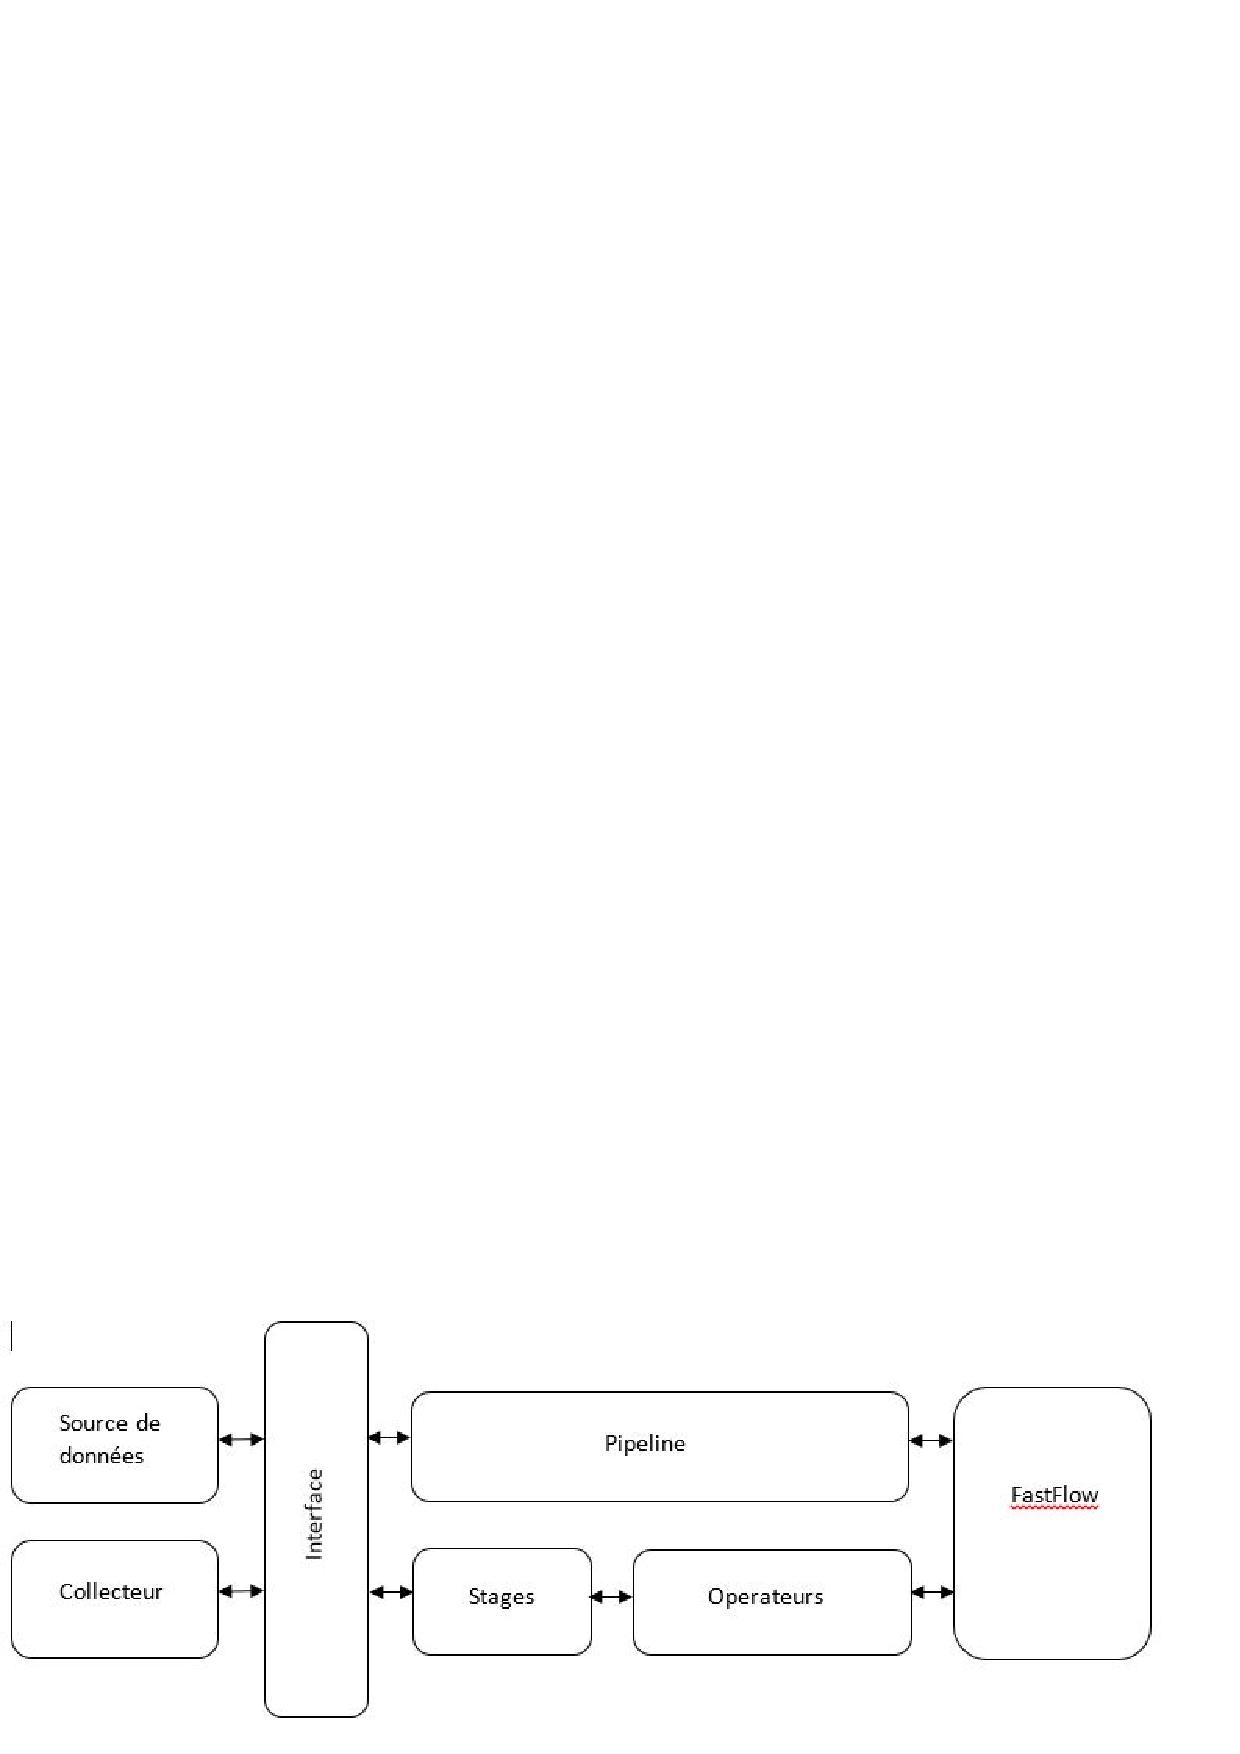
\includegraphics[width=1.0\textwidth]{Figures/ComponentsAPI.jpg}
      \caption{Components de l'API.}
       \label{ComponentsAPI.fig}
\end{figure}


\section{Les composants de l'API}

\subsection{Interface}

L'interface propos\'ee en PpFf consiste en un ensemble de m\'ethodes qui permettent \'a l'utilisateur de manipuler des flux de donn\'ees de mani\`ere simple et efficace. L'interface suit de pr\`es l'interface introduite dans la version Java Stream 8. Le tableau 3.1 d\'ecrit bri\`evement toutes les m\'ethodes impl\'ement\'es dans l'API.



\begin{figure}[h]
\centering

\resizebox{\textwidth}{!}{%

\begin{tabular}{|c|c|c|}
\hline
\textbf{M\'ethods} & \textbf{Retourn type} & \textbf{Description}\\
\hline
	\begin{tabular}{@{}l@{}}
	template<typename T> \\
	allMatch(std::function<bool(T*)> predicate)
	\end{tabular} &
  	bool & \begin{tabular}{@{}l@{}}
    Retourne vrais si tous les \'el\'ements \\ 
    de ce flux correspondent au pr\'edicat\\
    fourni.
    \end{tabular}\\
\hline
	\begin{tabular}{@{}l@{}}
	template<typename T> \\
	anyMatch(std::function<bool(T*)> predicate)
	\end{tabular} &
  	bool & \begin{tabular}{@{}l@{}}
    Retourne vrais si au moins un \\ 
    \'el\'ement de ce flux correspondent\\
    au pr\'edicat fourni.
    \end{tabular}\\
\hline
	\begin{tabular}{@{}l@{}}
	template < typename T, template \\
	<typename ELEM, class ALLOC = \\
	std::allocator<ELEM>> class TContainer >\\
	collect()
	\end{tabular} &
  	TContainer<T> & \begin{tabular}{@{}l@{}}
    Retourne un conteneur de type \\
    STL sur les \'el\'ements de ce flux.
    \end{tabular}\\
\hline
	\begin{tabular}{@{}l@{}}
	count()\\
	\end{tabular} &
  	unsigned int & \begin{tabular}{@{}l@{}}
    Retourne le nombre d'\'el\'ements \\
    dans ce flux.
    \end{tabular}\\
\hline
	\begin{tabular}{@{}l@{}}
	template<typename In> \\
	find(std::function<bool(In*)> const\& taskFunc)
	\end{tabular} &
  	Pipe\& & \begin{tabular}{@{}l@{}}
    Renvoie dans le flux tous les \\
    \'el\'ements qui satisfont la condition \\ 
    fournie en param\`etre.
    \end{tabular}\\
\hline
	\begin{tabular}{@{}l@{}}
	template<typename In, typename Out, \\
    typename OutContainer> \\
	flatMap(std::function<OutContainer*(In*)> \\
    const\& taskFunc)
	\end{tabular} &
  	Pipe\& & \begin{tabular}{@{}l@{}}
    Renvoie dans le flux le r\'esultat \\
    produit en appliquant la fonction \\
    de mappage fournie en param\`etre \\
    \`a chaque \'el\'ement.
    \end{tabular}\\
\hline
	\begin{tabular}{@{}l@{}}
	template<typename In, typename Out, \\
    typename OutContainer = In> \\
	flatMap()
	\end{tabular} &
  	Pipe\& & \begin{tabular}{@{}l@{}}
    Renvoie dans le flux les \\
    \'el\'ements du conteneur si \\
    celui-ci est un \'el\'ement du flux.
    \end{tabular}\\
\hline
	\begin{tabular}{@{}l@{}}
	template<typ name In, typename K = In, \\
    typename V = In, typename MapType> \\
	groupByKey(std::function<K*(In*)> const\& \\
    taskFuncOnKey, std::function<V*(In*)> \\
    const\& taskFuncOnValue = identity<In,V>)
	\end{tabular} &
  	MapType & \begin{tabular}{@{}l@{}}
    Retourne un map avec les \'el\'ements \\
    du flux groupés par cl\'e.
    \end{tabular}\\
\hline
%	\begin{tabular}{@{}l@{}}
%	template < typename T, \\
%    template <typename ELEM, class \\
%    ALLOC = std::allocator<ELEM>> \\
%    class TContainer > \\
%	intermediateCollect()
%	\end{tabular} &
%	Collection<T, TContainer, Pipe> & \begin{tabular}{@{}l@{}}
%    Retourne une collection avec les \\
%    \'el\'ements de ce flux.
%    \end{tabular}\\ 
%\hline
%	\begin{tabular}{@{}l@{}}
%	template<typename T> \\
%	limit (int n)
%	\end{tabular} &
%	Pipe\& & \begin{tabular}{@{}l@{}}
%    Renvoie dans le flux seulement \\
%    les n premiers \'el\'ements de \\
%    ce flux.
%    \end{tabular}\\
%\hline
%	\begin{tabular}{@{}l@{}}
%	linesFromFile(const std::string\& path)
%	\end{tabular} &
%	Pipe\& & \begin{tabular}{@{}l@{}}
%    Renvoie dans le flux les lignes \\
%    contenues dans un fichier.
%    \end{tabular}\\
%\hline
%	\begin{tabular}{@{}l@{}}
%	template<typename In, typename Out> \\
%	map(std::function<Out*(In*)> const\& \\ 
%    taskFunc)m	
%	\end{tabular} &
%	Pipe\& & \begin{tabular}{@{}l@{}}
%    Renvoie dans le flux les \\
%    r\'esultats constitu\'es de \\
%    l'application d'une fonction \\
%    fournie en param\`etre aux \\
%    \'el\'ements de ce flux.
%    \end{tabular}\\
%\hline

\end{tabular}
}
\caption{Les m\'ethodes expos\'ees aux utilisateurs par l'API.}
\label{methodes_api.tab}
\end{figure}

Comme on peut le voir dans le tableau 3.1, la d\'eclaration des m\'ethodes utilise la programmation g\'en\'erique de C++ qui sont les templates. Cela permet aux utilisateurs d'avoir une interface unique, de sorte qu'il peut \^etre r\'eutilis\'e pour n'importe quel type de donn\'ees.


Un autre point cl\'e dans cette interface le repr\'esente l'expressivit\'e. M\^eme avant de la conception, on s'est propos\'e de fournir un syst\`eme suffisamment intuitif et expressif pour le traitement de flux de donn\'ees. Le pseudocode 3.1 montre un extrait de code pour donner un premier aper\c{c}u de l'expressivit\'e de l'interface. D'autres exemples seront fournis plus tard dans ce document. Dans l'exemple fourni, on s\'electe seulement les employ\'ees qui ont un salaire plus grand que 35 milles. Les employ\'ees repr\'esent\'ees par un conteneur STL sont filtr\'ees en enchainant trois op\'erations : source qui a le r\^ole d'envoyer dans le flux les objets de type Employee, filtre qui filtre les employ\'ees selon la condition fournie en param\`etre et la derni\`ere op\'eration collect qui a le r\^ole de collecter les employ\'ees une fois filtr\'ees dans un conteneur STL. Dans cet exemple les employ\'ees sont ramass\'ees dans un conteneur de type vecteur. On note que le type de conteneur est donn\'e par le type fourni en param\`etre template de la m\'ethode collect.


\begin{pseudocode}
{\samepage\small
\begin{alltt}
std::vector<Employee> sourceEmployees;    
std::vector<Employee> result = 
        Pipe()
        .source<Employee>(sourceEmployees.begin(), sourceEmployees.end())
        .find<Employee>([](Employee *e) ->bool \{return e->salary > 35000;\})
        .collect<Employee, std::vector>();

\end{alltt}
}
\caption{L\'expressivit\'e de l'API.}
\label{expressivite_api.pseudo}
\end{pseudocode}




\subsection{Op\'erateurs}

Les op\'erateurs sont la base de notre syst\`eme. L'API fournit un ensemble d'op\'erateurs qui augmentent la productivit\'e de l'utilisateur. Les op\'erateurs sont structur\'es en deux cat\'egories : les op\'erateurs sans \'etat et op\'erateurs avec l'\'etat.

Les op\'erateurs sans \'etat sont les op\'erateurs qui ne disposent pas d'informations sur l'it\'eration en cours et ne transmettent pas les informations interm\'ediaires des \'etapes de traitement pr\'ec\'edentes. Si on prend comme exemple le filtre repr\'esent\'e par la m\'ethode find de le tableau 3.1, il traite le flux de donn\'ees \'el\'ement par \'el\'ement. Lorsque la fonction fournie en param\`etre de la m\'ethode find ne satisfait pas la condition de filtrage, le filtre ne retournera rien. Un op\'erateur sans \'etat, par contre il peut utiliser des donn\'ees historiques stock\'ees dans la m\'emoire locale ou sur le disque.

Les op\'erateurs avec l'\'etat sont les op\'erateurs qui maintiennent une structure de donn\'ees interne appel\'ee l'\'etat. Cette structure pr\'eserve l'historique des op\'erations pass\'ees et affecte la logique de traitement dans les calculs ult\'erieurs. Par exemple l'op\'erateur Sum calcule la somme des \'el\'ements du flux. Son \'etat contient la valeur de l'\'el\'ement en cours et la valeur de la somme de tous les \'el\'ements pr\'ec\'edents celui-ci. 



\subsection{Stages}

Le traitement du flux de donn\'ees est mod\'elis\'e en utilisant une cha\^{\i}ne d'\'etapes. Dans notre API, une \'etape est repr\'esent\'ee par un stage. Ce module n'est pas visible \`a l'utilisateur. Chaque stage est compos\'e d'un ou plusieurs op\'erateurs. 


\subsection{Pipeline}

Le pipeline est le composant principal de l'API. Un Pipeline est une cha\^{\i}ne de traitement compos\'ee d'un ou de plusieurs op\'erateurs group\'es dans des stages. La figure 3.2 montre une vue d\'etaill\'ee de pipeline en action. Une \'eétape de la cha\^{\i}ne de traitement de ce mod\`ele traite les donn\'ees produites par l'\'etape pr\'ec\'edente dans le flux et fournit les r\'esultats \`a l'étape suivante dans le flux. Un pipeline P avec n \'etapes peut \^etre formellement d\'efini comme :


{\small
\begin{alltt}
	P = O1 + O2 + O3 + … + On;
\end{alltt}
}

Dans l'expression ci-dessus O est repr\'esent\'e par le n-em op\'erateur dans le Pipeline.

L'utilisation de Pipeline introduit une couche d'abstraction sur une cha\^{\i}ne complexe d'op\'erateurs. De plus il n'expose pas à l'ext\'erieur que les entr\'ees et les sortirs du Pipeline. Une telle conception modulaire ajoute beaucoup de flexibilit\'e au syst\`eme tout en simplifiant la mise en œuvre. Par exemple, le parall\'elisme du flux pourrait \^etre facilement r\'ealis\'e en ayant plusieurs Pipelines identiques connect\'es \`a la m\^eme entr\'ee et sortie respectivement.


